% ================================================================================================
%  QLens: viva cheatsheet (RDBMS topics with real examples from the code, and a code map)
%  Build:  latexmk -pdf -jobname=QLens-Cheatsheet cheatsheet.tex   (or .\build.ps1 / make)
% ================================================================================================
\documentclass[10pt,a4paper]{article}
\usepackage[a4paper,left=1.1cm,right=1.1cm,top=1.0cm,bottom=1.35cm,footskip=0.6cm]{geometry}
\usepackage[T1]{fontenc}
\usepackage{lmodern}
\usepackage[sfdefault]{FiraSans}
\usepackage[scale=0.84]{FiraMono}
\usepackage{textcomp}
\usepackage{microtype}
\usepackage{xcolor}
\usepackage[most]{tcolorbox}
\usepackage{multicol}
\usepackage{listings}
\usepackage{tikz}
\usetikzlibrary{positioning,shapes.geometric,arrows.meta,calc,fit}
\usepackage{enumitem}
\usepackage{booktabs}
\usepackage{tabularx}
\usepackage{array}
\usepackage{amssymb}
\usepackage{fancyhdr}
\usepackage{lastpage}

% ---- colours: one per syllabus area ---------------------------------------------------------------
\definecolor{ink}{HTML}{1F2937}
\definecolor{muted}{HTML}{6B7280}
\definecolor{cIntro}{HTML}{1D4ED8}   % introduction, ER model
\definecolor{cRel}{HTML}{4338CA}     % relational model
\definecolor{cAlg}{HTML}{7E22CE}     % relational algebra
\definecolor{cSql}{HTML}{15803D}     % SQL
\definecolor{cAdv}{HTML}{C2410C}     % advanced SQL
\definecolor{cNorm}{HTML}{BE123C}    % normalization
\definecolor{cTx}{HTML}{A16207}      % transactions, concurrency
\definecolor{cSec}{HTML}{334155}     % security
\definecolor{cOpt}{HTML}{0F766E}     % optional / code map
\definecolor{codebg}{HTML}{F3F4F6}
\definecolor{kw}{HTML}{1E40AF}
\definecolor{cm}{HTML}{6B7280}
\definecolor{str}{HTML}{9A3412}
\definecolor{fileclr}{HTML}{374151}
\colorlet{boxc}{ink}

\color{ink}
\setlength{\parindent}{0pt}
\setlength{\columnsep}{0.45cm}
\setlength{\multicolsep}{2pt}
\raggedcolumns

% ---- page style -----------------------------------------------------------------------------------
\pagestyle{fancy}
\fancyhf{}
\renewcommand{\headrulewidth}{0pt}
\fancyfoot[L]{\fontsize{7}{8}\selectfont\color{muted}QLens viva cheatsheet \textperiodcentered{} Aditya Gaur, Aditya Choudhary}
\fancyfoot[R]{\fontsize{7}{8}\selectfont\color{muted}\thepage\ / \pageref{LastPage}}

% ---- inline helpers -------------------------------------------------------------------------------
% \code{...}: typewriter text in which % # _ $ ^ & ~ print as themselves (not inside other arguments).
\newcommand{\code}{\begingroup\catcode`\%=12 \catcode`\#=12 \catcode`\_=12 \catcode`\$=12
  \catcode`\^=12 \catcode`\&=12 \catcode`\~=12 \codeinner}
\newcommand{\codeinner}[1]{\texttt{#1}\endgroup}
% \ic|...|: inline code that may contain braces.
\lstdefinestyle{inl}{basicstyle=\ttfamily, columns=fullflexible, keepspaces=true, upquote=true}
\newcommand{\ic}{\lstinline[style=inl]}
\newcommand{\cd}[1]{\texttt{\detokenize{#1}}}
\newcommand{\fn}[1]{{\color{fileclr}\texttt{\detokenize{#1}}}}
\newcommand{\what}{{\color{boxc}\bfseries What.}\ }
\newcommand{\where}{{\color{boxc}\bfseries In QLens.}\ }
\newcommand{\ex}{{\color{boxc}\bfseries Example.}\ }
\newcommand{\why}{{\color{boxc}\bfseries Why.}\ }
\newcommand{\ra}{\ensuremath{\rightarrow}}
\newcommand{\opt}{\colorbox{cOpt!15}{\color{cOpt}\bfseries\fontsize{6.5}{7}\selectfont OPTIONAL}}

\setlist{nosep,leftmargin=0.95em,labelsep=0.35em,topsep=1pt}
\setlist[itemize]{label={\color{boxc}\textbullet}}
\setlist[enumerate]{label={\color{boxc}\bfseries\arabic*.}}

% ---- topic boxes ----------------------------------------------------------------------------------
\newtcolorbox{topic}[2][cIntro]{enhanced, colback=#1!3!white, colframe=#1, boxrule=0.6pt, arc=1.6pt,
  left=3.5pt, right=3.5pt, top=2.2pt, bottom=2.2pt, boxsep=0pt,
  title={#2}, fonttitle=\bfseries\fontsize{8.4}{9.8}\selectfont, coltitle=white, colbacktitle=#1,
  toptitle=1.3pt, bottomtitle=1.3pt, before skip=3.5pt, after skip=3.5pt,
  fontupper=\fontsize{7.9}{9.35}\selectfont,
  before upper={\colorlet{boxc}{#1}\setlength{\parskip}{1.6pt}\raggedright}}

\newcommand{\parthead}[3]{%
  \begin{tcolorbox}[enhanced, colback=ink, colframe=ink, arc=1.6pt, boxrule=0pt, left=6pt, right=6pt,
    top=3pt, bottom=3pt, before skip=2pt, after skip=4pt]
  {\color{white}\bfseries\fontsize{11}{13}\selectfont #1\quad}{\color{white!80!ink}\fontsize{8.5}{10}\selectfont #2}%
  \hfill{\color{white!70!ink}\fontsize{7.5}{9}\selectfont #3}
  \end{tcolorbox}}

% ---- code listings --------------------------------------------------------------------------------
\lstdefinestyle{base}{basicstyle=\fontsize{6.85}{8.0}\selectfont\ttfamily, columns=fullflexible,
  keepspaces=true, backgroundcolor=\color{codebg}, frame=none, xleftmargin=2pt, xrightmargin=2pt,
  framesep=0pt, aboveskip=2pt, belowskip=1pt, breaklines=true, breakatwhitespace=true,
  postbreak=\mbox{\textcolor{muted}{$\hookrightarrow$}\space}, showstringspaces=false, upquote=true,
  keywordstyle=\color{kw}\bfseries, commentstyle=\color{cm}\itshape, stringstyle=\color{str},
  tabsize=4}
\lstdefinestyle{sql}{style=base, language=SQL, morekeywords={RETURNING, GENERATED, IDENTITY, NULLS,
  EXCEPT, ALL, LATERAL, FILTER, CURSOR, FETCH, FORWARD, SCROLL, HOLD, TRIGGER, EXECUTE, FUNCTION,
  RETURNS, LANGUAGE, BEGIN, END, IF, THEN, ELSIF, ELSE, RETURN, EXCEPTION, WHEN, REVOKE, GRANT, ROLE,
  USAGE, SCHEMA, CASCADE, RESTRICT, REFERENCES, CONSTRAINT, STORED, ALWAYS, AFTER, BEFORE, EACH, ROW,
  DECLARE, NO, WITHOUT, LOGIN, PASSWORD, ALTER, VIEW, INDEX, WITH, FOR, STABLE, PUBLIC, BOOLEAN,
  BIGINT, TEXT, NUMERIC, DATE, OVER, LIMIT}, deletekeywords={MONTH}, sensitive=false}
\lstdefinestyle{py}{style=base, language=Python, morekeywords={with, as, None, True, False}}
\lstnewenvironment{sqlc}{\lstset{style=sql}}{}
\lstnewenvironment{pyc}{\lstset{style=py}}{}

\begin{document}
\fontsize{8.1}{9.6}\selectfont

% =================================================================================================
%  Title
% =================================================================================================
\begin{tcolorbox}[enhanced, colback=ink, colframe=ink, arc=2pt, boxrule=0pt, left=8pt, right=8pt,
  top=6pt, bottom=6pt, before skip=0pt, after skip=4pt,
  overlay={\fill[cIntro] ($(frame.south west)!0.0000!(frame.south east)$) rectangle ($(frame.south west)!0.1111!(frame.south east)+(0,2.4pt)$);
    \fill[cRel] ($(frame.south west)!0.1111!(frame.south east)$) rectangle ($(frame.south west)!0.2222!(frame.south east)+(0,2.4pt)$);
    \fill[cAlg] ($(frame.south west)!0.2222!(frame.south east)$) rectangle ($(frame.south west)!0.3333!(frame.south east)+(0,2.4pt)$);
    \fill[cSql] ($(frame.south west)!0.3333!(frame.south east)$) rectangle ($(frame.south west)!0.4444!(frame.south east)+(0,2.4pt)$);
    \fill[cAdv] ($(frame.south west)!0.4444!(frame.south east)$) rectangle ($(frame.south west)!0.5556!(frame.south east)+(0,2.4pt)$);
    \fill[cNorm] ($(frame.south west)!0.5556!(frame.south east)$) rectangle ($(frame.south west)!0.6667!(frame.south east)+(0,2.4pt)$);
    \fill[cTx] ($(frame.south west)!0.6667!(frame.south east)$) rectangle ($(frame.south west)!0.7778!(frame.south east)+(0,2.4pt)$);
    \fill[cSec] ($(frame.south west)!0.7778!(frame.south east)$) rectangle ($(frame.south west)!0.8889!(frame.south east)+(0,2.4pt)$);
    \fill[cOpt] ($(frame.south west)!0.8889!(frame.south east)$) rectangle ($(frame.south west)!1.0000!(frame.south east)+(0,2.4pt)$);}]
{\color{white}\bfseries\fontsize{19}{22}\selectfont QLens \textperiodcentered{} Viva Cheatsheet}\par\smallskip
{\color{white!85!ink}\fontsize{9}{11}\selectfont QLens: An Automated Relational Database Design and Normalization System}\par\smallskip
{\color{white!70!ink}\fontsize{8}{10}\selectfont Aditya Gaur \,\textperiodcentered\, Aditya Choudhary
\quad|\quad CSC2103 Relational Database Management Systems \,\textperiodcentered\, B.Tech CSE, Semester III
\,\textperiodcentered\, Manipal University Jaipur}
\end{tcolorbox}

\begin{tcolorbox}[colback=codebg, colframe=codebg, arc=1.6pt, left=5pt, right=5pt, top=2.5pt, bottom=2.5pt,
  before skip=0pt, after skip=3pt, fontupper=\fontsize{7.6}{9.2}\selectfont]
\textbf{How to read.} Each box: \textbf{What} (one-line definition) \textperiodcentered{} \textbf{In QLens}
(screen + file) \textperiodcentered{} a real snippet. Python paths are under \fn{backend/qlens/}, e.g.\
\fn{design/ddl.py:_create_table L86}. SQL migrations are cited as \fn{001:212} =
\fn{backend/sql/migrations/001_schema.sql} line 212. \code{ws_20} = workspace number 20 (any id works).
Snippets are copied from the code; long lines are re-wrapped and \code{...} marks lines left out.
\textbf{Areas:}
\textcolor{cIntro}{\rule{6pt}{6pt}} Intro \& ER\enspace
\textcolor{cRel}{\rule{6pt}{6pt}} Relational model\enspace
\textcolor{cAlg}{\rule{6pt}{6pt}} Relational algebra\enspace
\textcolor{cSql}{\rule{6pt}{6pt}} SQL\enspace
\textcolor{cAdv}{\rule{6pt}{6pt}} Advanced SQL\enspace
\textcolor{cNorm}{\rule{6pt}{6pt}} Normalization\enspace
\textcolor{cTx}{\rule{6pt}{6pt}} Transactions\enspace
\textcolor{cSec}{\rule{6pt}{6pt}} Security\enspace
\textcolor{cOpt}{\rule{6pt}{6pt}} Optional / code map
\end{tcolorbox}

\parthead{PART A}{RDBMS topics in QLens}{one box per syllabus topic}

\begin{multicols}{2}

% -------------------------------------------------------------------------------------------------
\begin{topic}[cIntro]{File system vs DBMS: the spreadsheet problem}
\what A spreadsheet (flat file) repeats the same fact on many rows and checks nothing. A DBMS stores
each fact once, enforces rules (constraints), controls concurrent users and recovers after a crash.

\ex The \textbf{fee register} sample: 3{,}000 rows = 300 students $\times$ 10 months, columns
Student Name, Student Phone, Batch, Teacher, Teacher Phone, Month, Fee Paid, Payment Mode.
\begin{itemize}
  \item \textbf{Update anomaly:} a teacher's phone is copied on every row of the batch. The sample has
  Mr.\ Gupta's \emph{old} number in exactly 5 rows: one fact, two values.
  \item \textbf{Insertion anomaly:} a new batch and its teacher cannot be stored until some student of
  that batch has a fee row.
  \item \textbf{Deletion anomaly:} deleting the last fee rows of a batch also loses who teaches it.
\end{itemize}
\where Import keeps the sheet as it is (\code{ws_<id>_src._raw}); Analyze finds the repetition
(functional dependencies); Design splits it into \code{teachers}, \code{batches}, \code{students},
\code{fee_register}, so each fact is stored once.
\end{topic}

% -------------------------------------------------------------------------------------------------
\begin{topic}[cIntro]{Schema, instance, data independence}
\what \textbf{Schema} = the design (tables, columns, types, constraints), changes rarely.
\textbf{Instance} = the rows at one moment. \textbf{Data independence} = changing one level does not
break the level above it.
\begin{itemize}
  \item A design (schema) is stored as \emph{data} in \code{qlens.schema_proposals},
  \code{proposed_tables}, \code{proposed_columns}; the instance is the rows of \code{ws_20.students} etc.
  \item The \textbf{system catalog} (data dictionary) is read by \fn{design/catalog.py:describe L56}:
  \code{pg_class}, \code{pg_attribute}, \code{pg_constraint}, \code{pg_index}.
  \item Three levels: external = views (\code{original_sheet}, \code{v_workspace_summary}); conceptual
  = tables; physical = heap files and B-tree indexes.
  \item \textbf{Logical} independence: after Apply the sheet is 4 tables, yet
  \code{SELECT * FROM original_sheet} still returns the old sheet columns.
  \item \textbf{Physical} independence: ``Explain \& speed up'' adds an index; the same SELECT text
  just runs faster.
\end{itemize}
\end{topic}

% -------------------------------------------------------------------------------------------------
\begin{topic}[cIntro]{DBMS architecture and users}
\what Three-tier: client $\to$ application server $\to$ database server.
\where Browser (React) $\to$ FastAPI (Python, \code{/api/...}) $\to$ PostgreSQL 18 (diagram in Part B).
Users: \textbf{naive} users click through Import/Analyze/Design; \textbf{sophisticated} users type SQL in
Data $>$ SQL; \textbf{application programmers} (us) wrote every SQL statement by hand (no ORM);
the \textbf{DBA} step is \fn{setup_db.py} (creates role \code{qlens_app}, the database and the
\code{pg_trgm} extension) and \fn{migrate.py} (runs \code{000}--\code{008}, records them in
\code{qlens.schema_migrations}). Applications: fee registers, shop bills, hostel mess (the three samples
in \fn{samples/generate.py}).
\end{topic}

% -------------------------------------------------------------------------------------------------
\begin{topic}[cIntro]{ER model: entities, attributes, relationships}
\what Entity set (rectangle), attribute (ellipse; key underlined), relationship set (diamond),
cardinality 1\,:\,1, 1\,:\,N, M\,:\,N. Attributes: simple/composite, single/multivalued, stored/derived.
\where The \code{qlens} schema itself: User \emph{owns} (1\,:\,N) Workspace \emph{holds} (1\,:\,1)
Dataset \emph{has} (1\,:\,N) Column; Functional Dependency \emph{LHS} (M\,:\,N) Column; Dataset
\emph{proposes} (1\,:\,N) Schema Proposal \emph{contains} (1\,:\,N) Proposed Table. Sketch in Part B.
\begin{itemize}
  \item \textbf{Derived attribute}, computed by PostgreSQL (\fn{001:136}):
\end{itemize}
\begin{sqlc}
is_exact        boolean GENERATED ALWAYS AS (violating_rows = 0) STORED,
violation_ratio numeric GENERATED ALWAYS AS
    (violating_rows::numeric / NULLIF(row_count, 0)) STORED,
\end{sqlc}
\begin{itemize}
  \item \textbf{Multivalued attribute}: an FD's left side can have 2 columns $\to$ rows of
  \code{fd_lhs_columns}, never a list inside one cell.
  \item \textbf{Weak entity}: \code{duplicate_values(group_id, value)} has no own id; partial key
  \code{value} + owner \code{duplicate_groups} (\fn{001:172}).
  \item \textbf{Specialization} as a type attribute: \code{proposed_tables.kind IN ('entity','fact')},
  \code{proposed_columns.role IN ('pk','fk','attribute')}.
\end{itemize}
\end{topic}

% -------------------------------------------------------------------------------------------------
\begin{topic}[cIntro]{ER $\to$ relational mapping (the 4 rules)}
\begin{enumerate}
  \item Strong entity set $\to$ table, its key $\to$ \code{PRIMARY KEY}: \code{users(id, email, ...)} (\fn{001:33}).
  \item 1\,:\,N $\to$ foreign key on the N side: \code{workspaces.owner_id REFERENCES users(id)} (\fn{001:61}).
  \item 1\,:\,1 $\to$ foreign key + \code{UNIQUE}: \code{datasets.workspace_id ... UNIQUE} (\fn{001:72}).
  \item M\,:\,N $\to$ its own table, primary key = both foreign keys:
\end{enumerate}
\begin{sqlc}
CREATE TABLE qlens.fd_lhs_columns (                        -- 001:148
    fd_id     bigint NOT NULL REFERENCES
              qlens.functional_dependencies (id) ON DELETE CASCADE,
    column_id bigint NOT NULL REFERENCES
              qlens.dataset_columns (id) ON DELETE CASCADE,
    PRIMARY KEY (fd_id, column_id)
);
\end{sqlc}
Also M\,:\,N: \code{candidate_key_columns}, \code{proposed_unique_key_columns}. Result: 26 tables in
schema \code{qlens} (+ \code{schema_migrations}). The user's data follows the same rules: Teacher 1\,:\,N
Batch 1\,:\,N Student 1\,:\,N fee row $\to$ \code{batches.teacher_id}, \code{students.batch_id},
\code{fee_register.student_id}.
\end{topic}

% -------------------------------------------------------------------------------------------------
\begin{topic}[cRel]{Relation, tuple, attribute, domain}
\what Relation = table, tuple = row, attribute = column, \textbf{domain} = set of allowed values (type +
CHECK). Degree = number of columns; cardinality = number of rows.
\where On Import the database itself decides each column's domain:
\fn{ingest/stage.py:_infer_type L97} picks the first of integer, numeric, boolean, date that fits every
non-empty value, else text:
\begin{sqlc}
SELECT bool_and({c} ~ %(int)s) AS is_int,
       bool_and({c} ~ %(num)s) AS is_num,
       bool_and(lower({c}) = ANY(%(bools)s)) AS is_bool,
       bool_and(CASE WHEN {c} ~ %(dateish)s
           THEN qlens.try_date({c}) IS NOT NULL ELSE false END)
       AS is_date
FROM {t} WHERE {c} IS NOT NULL
\end{sqlc}
Then \fn{_build_staging L140} runs \code{CREATE TABLE _staging AS SELECT _row_id, ...} with casts
(\code{fee_paid::bigint}). Phones like ``+91 98765 43210'' stay \code{text}. A domain as a CHECK:
\code{inferred_type IN ('integer','numeric','boolean','date','text')} (\fn{001:91}).
\end{topic}

% -------------------------------------------------------------------------------------------------
\begin{topic}[cRel]{Keys: super, candidate, primary, foreign; surrogate vs natural}
\what \textbf{Superkey}: columns whose values differ in every row. \textbf{Candidate key}: a minimal
superkey. \textbf{Primary key}: the chosen one (others = alternate keys). \textbf{Foreign key}: refers to
a key of another table. \textbf{Surrogate} key = a number made by the system (\code{id});
\textbf{natural} key = from the data (\code{email}, \code{student_name}).
\where Analyze $\to$ \fn{analysis/discover.py:_find_keys L69} tries 1-, 2-, 3-column sets:
\begin{pyc}
if any(set(k) <= set(names) for k in keys):
    return False   # a superset of a smaller key is not a new key
if any(c.null_count > 0 for c in combo):
    return False   # a key must be filled in on every row
if math.prod(c.distinct_count for c in combo) < row_count:
    return False   # cannot be unique: never reaches the database
return bool(conn.execute(
    "SELECT qlens.is_unique(%s, '_staging', %s) AS u",
    (schema, list(names))).fetchone()["u"])
\end{pyc}
Fee register: candidate key e.g.\ \{student\_name, month\}. Generated tables get a surrogate
\code{id bigint GENERATED ALWAYS AS IDENTITY PRIMARY KEY} and keep the natural key as \code{UNIQUE}
(\fn{design/ddl.py:_create_table L90, L98}).
\end{topic}

% -------------------------------------------------------------------------------------------------
\begin{topic}[cRel]{Integrity constraints}
\what Rules the DBMS enforces on every change: domain (type, CHECK), entity integrity (primary key is
unique and not null), key (UNIQUE), referential integrity (FOREIGN KEY).
\begin{sqlc}
email text NOT NULL UNIQUE                                 -- 001:36
      CHECK (email = lower(email) AND position('@' in email) > 1),
UNIQUE (owner_id, name)                                    -- 001:66
CHECK ((status = 'ok') = (error_message IS NULL))          -- 001:313
CHECK (status <> 'applied' OR lossless_ok IS TRUE)         -- 001:212
\end{sqlc}
\begin{itemize}
  \item \textbf{Why \code{IS TRUE}}: a CHECK \emph{passes} when it is NULL (unknown). \code{lossless_ok}
  is NULL until the check runs; \code{lossless_ok = true} would let an unchecked design become
  ``applied''. \code{NULL IS TRUE} is false, so it is refused.
  \item \textbf{\code{UNIQUE NULLS NOT DISTINCT}} on generated tables (\fn{ddl.py L98}): two NULLs
  normally never clash; here an empty natural key (no teacher) is one value, stored once.
  \item \textbf{FK actions}: \code{ON DELETE CASCADE} deleting a user deletes their workspaces, datasets\dots{}
  (\fn{001:61}); \code{SET NULL} deleting a saved query keeps its run history (\fn{001:303});
  \code{RESTRICT} on generated FKs: a student with fee rows cannot be deleted (\fn{ddl.py L102}).
\end{itemize}
\end{topic}

% -------------------------------------------------------------------------------------------------
\begin{topic}[cAlg]{Relational algebra: the ``Step through'' button}
\what Unary: $\sigma$ selection (rows), $\pi$ projection (columns), $\rho$ rename. Binary: $\times$
product, $\bowtie$ join, $\cup$, $\cap$, $-$. Extended: $\gamma$ grouping, $\delta$ duplicate
elimination, $\tau$ sort.
\where Data $>$ SQL $>$ Step through $\to$ \fn{stepthrough/stages.py:_build L208} cuts one SELECT into a
chain of runnable SELECTs, one per operator, runs each in the sandbox and shows the rows after each step:

\smallskip
{\setlength{\tabcolsep}{3pt}\renewcommand{\arraystretch}{1.05}
\begin{tabular}{@{}l l l l@{}}
\toprule
FROM \dots JOIN & $\bowtie$ join & GROUP BY & $\gamma$ grouping\\
FROM a, b & $\times$ product & HAVING & $\sigma$ on groups\\
WHERE & $\sigma$ selection & SELECT & $\pi$ projection\\
DISTINCT & $\delta$ & ORDER BY/LIMIT & $\tau$ sort\\
\bottomrule
\end{tabular}}
\begin{sqlc}
SELECT b.batch, count(*) AS unpaid
FROM fee_register f JOIN students s ON s.id = f.student_id
                    JOIN batches  b ON b.id = s.batch_id
WHERE f.fee_paid = 0
GROUP BY b.batch HAVING count(*) > 25;
\end{sqlc}
$= \pi_{\textit{batch, unpaid}}\big(\sigma_{\textit{count}>25}\big(\gamma_{\textit{batch};\,\textit{count(*)}}
\big(\sigma_{\textit{fee\_paid}=0}(F \bowtie S \bowtie B)\big)\big)\big)$.
UNION/INTERSECT/EXCEPT are refused here (\fn{stages.py:_parse}): they combine two whole queries.
\end{topic}

% -------------------------------------------------------------------------------------------------
\begin{topic}[cAlg]{Set difference: EXCEPT ALL in the lossless check}
\what $r - s$ = tuples of $r$ that are not in $s$. SQL \code{EXCEPT} is set difference;
\code{EXCEPT ALL} is the multiset (bag) version that also counts repeated rows.
\where Apply $\to$ \fn{design/ddl.py:_verify L220} (schemas left out; \code{cols} = the 8 sheet columns):
\begin{sqlc}
SELECT (SELECT count(*) FROM _staging)       AS staging_rows,
       (SELECT count(*) FROM original_sheet) AS reconstructed_rows,
       (SELECT count(*) FROM (SELECT cols FROM original_sheet
            EXCEPT ALL SELECT cols FROM _staging) d)       AS extra_rows,
       (SELECT count(*) FROM (SELECT cols FROM _staging
            EXCEPT ALL SELECT cols FROM original_sheet) d) AS missing_rows
\end{sqlc}
Both differences 0 $\Rightarrow$ joining the new tables gives back exactly the sheet. \why\ \code{ALL}:
with plain EXCEPT a row that is in the sheet twice but rebuilt once would go unnoticed.
\end{topic}

% -------------------------------------------------------------------------------------------------
\begin{topic}[cSql]{DDL: CREATE / ALTER / DROP}
\where
\begin{itemize}
  \item \code{CREATE SCHEMA ws_20}, \code{ws_20_src}, \code{ws_20_lab} and \code{DROP SCHEMA ... CASCADE}:
  \fn{db.py:create_ws_schema}, \fn{drop_ws_schema}.
  \item \code{CREATE TABLE ... AS SELECT} (typed copy) + \code{ALTER TABLE ... ADD PRIMARY KEY}:
  \fn{ingest/stage.py:_build_staging L140}.
  \item The design's script (Design $>$ SQL panel): \fn{design/ddl.py:render L235} = schema, tables
  (referenced tables first), loads, triggers, view, verify. Real output for the fee register:
\end{itemize}
\begin{sqlc}
CREATE TABLE ws_20.fee_register (
    id bigint GENERATED ALWAYS AS IDENTITY PRIMARY KEY,
    student_id bigint NOT NULL,
    month text NOT NULL,
    fee_paid bigint NOT NULL,
    payment_mode text,
    CONSTRAINT fee_register_student_id_month_key
        UNIQUE NULLS NOT DISTINCT (student_id, month),
    CONSTRAINT fee_register_student_id_fkey FOREIGN KEY (student_id)
        REFERENCES ws_20.students (id) ON DELETE RESTRICT
);
\end{sqlc}
\code{CREATE VIEW original_sheet} (\fn{ddl.py:_view L159}); \code{CREATE INDEX} (\fn{perf/lab.py:try_index L239});
\code{CREATE TRIGGER} (\fn{ddl.py:_audit_trigger L107}).
\end{topic}

% -------------------------------------------------------------------------------------------------
\begin{topic}[cSql]{DML: INSERT, UPDATE, DELETE, COPY}
\where
\begin{itemize}
  \item Import: \code{COPY ws_20_src._raw (...) FROM STDIN} (\fn{ingest/stage.py:92}), then
  \code{INSERT INTO qlens.datasets / dataset_columns}.
  \item Apply fills each table with \code{INSERT ... SELECT} from \code{_staging}
  (\fn{design/ddl.py:_load L121}); entity tables use \code{DISTINCT}; a foreign key is looked up by
  joining the parent on its natural key:
\end{itemize}
\begin{sqlc}
INSERT INTO ws_20.students (student_name, student_phone, batch_id)
SELECT DISTINCT s.student_name, s.student_phone, batches.id
FROM ws_20_src._staging s
LEFT JOIN ws_20.batches ON batches.batch = s.batch
ORDER BY 1, 2, 3
\end{sqlc}
\begin{itemize}
  \item Clean-up: \code{UPDATE _staging} (\fn{analysis/cleanup.py:_rewrite L219}).
  \item Data $>$ Browse: \fn{data/service.py:insert_row L407}, \fn{update_row L420},
  \fn{delete_row L435}, e.g.\ \ic|UPDATE {} SET {} WHERE id = %s RETURNING {}| (each SET part is \ic|{} = %s|).
  \item Data $>$ SQL: one typed INSERT/UPDATE/DELETE (\fn{query/routes.py:run_write L188}).
\end{itemize}
\end{topic}

% -------------------------------------------------------------------------------------------------
\begin{topic}[cSql]{DCL: roles, GRANT, REVOKE}
\what DCL gives or takes away privileges. \where \fn{workspaces/service.py:create_workspace L71} and
\fn{db.py:create_ws_schema}, \fn{grant_ws_writes}; shown as the SQL they send for workspace 20:
\begin{sqlc}
CREATE ROLE qlens_ws_20 LOGIN PASSWORD '...'
    NOINHERIT CONNECTION LIMIT 3;
ALTER ROLE qlens_ws_20 SET statement_timeout = '5s';
ALTER ROLE qlens_ws_20 SET default_transaction_read_only = on;
GRANT USAGE ON SCHEMA ws_20 TO qlens_ws_20;
GRANT SELECT ON ALL TABLES IN SCHEMA ws_20 TO qlens_ws_20;
GRANT INSERT, UPDATE, DELETE ON ALL TABLES IN SCHEMA ws_20
    TO qlens_ws_20;                         -- main schema only
REVOKE INSERT, UPDATE, DELETE ON ws_20.original_sheet
    FROM qlens_ws_20;                       -- views stay read-only
REVOKE EXECUTE ON FUNCTION qlens.log_row_change()
    FROM PUBLIC;                            -- 007:9
\end{sqlc}
\code{ALTER DEFAULT PRIVILEGES} gives tables created later the same rights. The role's password is
derived (HMAC of the secret key), never stored (\fn{db.py:ws_password}).
\end{topic}

% -------------------------------------------------------------------------------------------------
\begin{topic}[cSql]{Joins}
\what Inner join keeps matching rows; left outer join keeps every left row (NULLs when no match);
self join joins a table with itself; lateral join lets the right side use the left row.
\where Reading an FD with its column names, \fn{analysis/discover.py:_FD_SQL L197}:
\begin{sqlc}
SELECT f.id, rc.name AS rhs,
       array_agg(lc.name ORDER BY lc.ordinal) AS lhs, ...
FROM qlens.functional_dependencies f
JOIN qlens.dataset_columns rc ON rc.id = f.rhs_column_id
JOIN qlens.fd_lhs_columns l   ON l.fd_id = f.id
JOIN qlens.dataset_columns lc ON lc.id = l.column_id
WHERE f.dataset_id = %(ds)s
GROUP BY f.id, rc.name, rc.label, rc.ordinal
\end{sqlc}
\begin{itemize}
  \item \code{original_sheet}: \code{fee_register LEFT JOIN students LEFT JOIN batches LEFT JOIN teachers}
  (\fn{ddl.py:_view}).
  \item Self join: \code{FROM c a JOIN c b ON a.norm = b.norm AND a.val < b.val} pairs two spellings of
  the same value (\fn{cleanup.py:_column_clusters L115}).
  \item \code{LEFT JOIN LATERAL} in \code{v_workspace_summary} (\fn{002:70}).
\end{itemize}
\end{topic}

% -------------------------------------------------------------------------------------------------
\begin{topic}[cSql]{Subqueries}
\what A query inside a query: scalar (one value), in \code{IN}/\code{EXISTS}, in \code{FROM} (derived
table), correlated (uses the outer row); \code{WITH} names one (CTE).
\where
\begin{itemize}
  \item Scalar + derived-table subqueries: the lossless check above; \code{is_unique}:
  \code{SELECT count(*) FROM (SELECT DISTINCT cols FROM t) d} (\fn{004:43}).
  \item \code{IN} subquery: Browse search finds a fee row by its student's name
  (\fn{data/service.py:_view L179}):
  \code{t.student_id IN (SELECT r.id FROM ws_20.students r WHERE <name> ILIKE %s)}.
  \item CTEs: \code{check_fd}, \code{v_slow_queries}, \code{cleanup._rewrite}.
  \item Correlated \code{NOT EXISTS}, to run in Data $>$ SQL (students who never missed a payment):
\end{itemize}
\begin{sqlc}
SELECT s.student_name FROM students s
WHERE NOT EXISTS (SELECT 1 FROM fee_register f
                  WHERE f.student_id = s.id AND f.fee_paid = 0);
\end{sqlc}
\end{topic}

% -------------------------------------------------------------------------------------------------
\begin{topic}[cSql]{Views}
\what A virtual table: a stored query, no stored rows.
\where \code{v_workspace_summary} (\fn{002:54}, dashboard cards), \code{v_slow_queries} (\fn{002:84},
History: runs above the workspace's 90th percentile via \code{percentile_cont(0.9)}),
\code{v_saved_query_trend} (\fn{002:112}, window functions \code{row_number()}, \code{lag()},
\code{avg() OVER (... ROWS BETWEEN 4 PRECEDING AND CURRENT ROW)}). Per workspace,
\fn{design/ddl.py:_view L159} rebuilds the sheet:
\begin{sqlc}
CREATE VIEW ws_20.original_sheet AS
SELECT students.student_name, students.student_phone, batches.batch,
       teachers.teacher, teachers.teacher_phone, fee_register.month,
       fee_register.fee_paid, fee_register.payment_mode
FROM ws_20.fee_register
LEFT JOIN ws_20.students ON students.id = fee_register.student_id
LEFT JOIN ws_20.batches ON batches.id = students.batch_id
LEFT JOIN ws_20.teachers ON teachers.id = batches.teacher_id
\end{sqlc}
\end{topic}

% -------------------------------------------------------------------------------------------------
\begin{topic}[cSql]{Aggregation: GROUP BY, HAVING}
\what Aggregate functions (\code{count}, \code{sum}, \code{max}, \code{avg}) summarize each group;
\code{HAVING} filters whole groups.
\where The FD test \code{qlens.check_fd} (\fn{004:14}) is two GROUP BYs (placeholders \code{%1$s},
\code{%2$I} written as \code{lhs}, \code{rhs}):
\begin{sqlc}
WITH c AS (SELECT lhs, rhs, count(*) AS cnt
           FROM t GROUP BY lhs, rhs),
     g AS (SELECT lhs, sum(cnt) AS n, max(cnt) AS keep
           FROM c GROUP BY lhs)
SELECT (SELECT count(*) FROM t),              -- row_count
       count(*),                              -- lhs_values
       count(*) FILTER (WHERE n >= 2),        -- repeated_groups
       coalesce(sum(n - keep), 0)::bigint     -- violating_rows
FROM g
\end{sqlc}
\ex teacher $\to$ teacher\_phone: in Mr.\ Gupta's group $n$ = all his rows, \code{keep} = rows with the
common number, so $n - \textit{keep} = 5$ (the old number) $\Rightarrow$ 5 violating rows. batch
$\to$ teacher: every group has one teacher $\Rightarrow$ 0 (exact).
\end{topic}

% -------------------------------------------------------------------------------------------------
\begin{topic}[cAdv]{Triggers (OLD / NEW)}
\what A procedure the DBMS runs by itself on INSERT/UPDATE/DELETE: BEFORE or AFTER, FOR EACH ROW;
\code{OLD} = row before, \code{NEW} = row after.
\begin{enumerate}
  \item \code{touch_updated_at}: BEFORE UPDATE, \code{NEW.updated_at := clock_timestamp()}
  (\fn{002:11}; on workspaces, datasets, saved\_queries, assistant\_conversations).
  \item \code{record_query_run}: AFTER INSERT ON query\_runs \code{WHEN (NEW.saved_query_id IS NOT NULL AND
  NEW.status = 'ok')} $\to$ \code{run_count + 1} (\fn{002:29--43}).
  \item \code{log_row_change}: audit log of every change on the generated tables (\fn{006:24}),
  attached by Apply \emph{after} the loads (\fn{ddl.py:_audit_trigger L107}):
\end{enumerate}
\begin{sqlc}
IF TG_OP IN ('UPDATE', 'DELETE') THEN old_row := to_jsonb(OLD); END IF;
IF TG_OP IN ('INSERT', 'UPDATE') THEN new_row := to_jsonb(NEW); END IF;
INSERT INTO qlens.row_changes
       (workspace_id, table_name, op, row_pk, before, after)
VALUES (ws_id, TG_TABLE_NAME, TG_OP,
        (coalesce(new_row, old_row) ->> 'id')::bigint,
        old_row, new_row);
RETURN NULL;   -- the result of an AFTER trigger is ignored
-- attached to each generated table:
CREATE TRIGGER log_row_change AFTER INSERT OR UPDATE OR DELETE
    ON ws_20.students FOR EACH ROW
    EXECUTE FUNCTION qlens.log_row_change();
\end{sqlc}
\why\ a trigger: it catches every change (Browse forms, typed SQL, anything) inside the same
transaction; no code path can forget it. \code{SECURITY DEFINER} (\fn{007:7}) lets it write
\code{qlens.row_changes} even when the sandbox role made the change.
\end{topic}

% -------------------------------------------------------------------------------------------------
\begin{topic}[cAdv]{Cursors}
\what A cursor points into a query's result so rows can be read a few at a time: \code{DECLARE},
\code{FETCH}, \code{CLOSE} (or end of transaction).
\where Every SELECT from Data $>$ SQL, each step-through stage and Ask AI's \code{run_sql} go through
\fn{query/sandbox.py:run}:
\begin{pyc}
_CURSOR = "qlens_run"
_DECLARE = f"DECLARE {_CURSOR} NO SCROLL CURSOR WITHOUT HOLD FOR "
...
conn.execute(_DECLARE + sql_text, prepare=True)
cur = conn.execute(f"FETCH FORWARD {int(max_rows) + 1} FROM {_CURSOR}")
\end{pyc}
It fetches 1{,}001 rows: 1{,}000 are shown, the extra one only says ``truncated''. A huge result never
sits in memory. \code{NO SCROLL} = forward only; \code{WITHOUT HOLD} = closed when the (rolled-back)
transaction ends. PL/pgSQL also uses an implicit cursor: \code{FOR t IN SELECT ... LOOP} in \fn{006:47--61}.
\end{topic}

% -------------------------------------------------------------------------------------------------
\begin{topic}[cAdv]{Stored procedures / functions (PL/pgSQL)}
\what A named program stored in the database and called from SQL; PL/pgSQL adds variables, IF,
loops and exception handling. (In PostgreSQL these are functions, called with SELECT.)
\where \code{check_fd(schema, table, lhs text[], rhs) RETURNS TABLE (...)} (\fn{004:14}) and
\code{is_unique(schema, table, cols text[]) RETURNS boolean} (\fn{004:33}), both called from
\fn{analysis/discover.py}; and \code{try_date} (\fn{003:8}):
\begin{sqlc}
CREATE FUNCTION qlens.try_date(p text) RETURNS date
LANGUAGE plpgsql STABLE AS $$
BEGIN
    IF p ~ '^\d{4}-\d{2}-\d{2}$' THEN
        RETURN p::date;
    ELSIF p ~ '^\d{1,2}[/-]\d{1,2}[/-]\d{4}$' THEN
        RETURN to_date(replace(p, '-', '/'), 'DD/MM/YYYY');
    END IF;
    RETURN NULL;
EXCEPTION WHEN others THEN
    RETURN NULL;          -- 31/02/2026 gives NULL, not an error
END;
$$;
\end{sqlc}
Dynamic SQL is safe: table and column names go through \code{format('%I')} (quoted identifiers).
\end{topic}

% -------------------------------------------------------------------------------------------------
\begin{topic}[cAdv]{Indexing (B-tree) and ``Explain \& speed up''}
\what An index (PostgreSQL's default is a B$^{+}$-tree, called \code{btree}) finds rows without scanning
the whole table; it costs space and slows writes. PRIMARY KEY/UNIQUE create one automatically; others
are \textbf{secondary} indexes. Each one in \fn{001} has a comment naming the query it serves:
\begin{sqlc}
CREATE INDEX query_runs_workspace_time_idx               -- 001:317
    ON qlens.query_runs (workspace_id, created_at DESC); -- History
CREATE INDEX query_runs_saved_query_time_idx             -- 001:320
    ON qlens.query_runs (saved_query_id, created_at)
    WHERE saved_query_id IS NOT NULL;                    -- partial
CREATE INDEX sessions_user_id_idx ON qlens.sessions (user_id);
                     -- 001:53, FK column: serves ON DELETE CASCADE
\end{sqlc}
PostgreSQL does not index foreign keys by itself, so 001 adds them. A \textbf{GIN} trigram index finds
look-alike spellings: \code{CREATE INDEX ON pg_temp._qlens_vals USING gin (val gin_trgm_ops)}
(\fn{cleanup.py:147}).

\where Data $>$ SQL $>$ Explain \& speed up $\to$ \fn{perf/lab.py:try_index L205}: median of 5
\code{EXPLAIN ANALYZE} runs $\to$ \code{CREATE INDEX} on a lab copy $\to$ \code{ANALYZE} $\to$ 5 runs
again $\to$ row in \code{qlens.index_experiments} (\code{speedup} = before/after, generated column).
\ex \code{SELECT * FROM fee_register WHERE fee_paid = 2100}: Seq Scan before, index on
\code{(fee_paid)} after.
\end{topic}

% -------------------------------------------------------------------------------------------------
\begin{topic}[cNorm]{Functional dependencies (exact vs approximate)}
\what $X \to A$: any two rows with the same $X$ have the same $A$ (trivial if $A \in X$).
\textbf{Exact}: holds in every row. \textbf{Approximate}: broken in a few rows (QLens: at most 2\%,
\code{APPROX_THRESHOLD = 0.02}, \fn{discover.py:16}), usually a typing mistake.
\where Analyze $\to$ \fn{analysis/discover.py:_find_fds L97} runs \code{check_fd} for single columns,
then pairs:
\begin{pyc}
m = conn.execute("SELECT * FROM qlens.check_fd(%s, '_staging', %s, %s)",
                 (schema, names, rhs)).fetchone()
if m["repeated_groups"] >= 2 and \
   m["violating_rows"] <= APPROX_THRESHOLD * m["row_count"]:
    return {"lhs": names, "rhs": rhs, **m}
\end{pyc}
\ex batch $\to$ teacher (exact); student\_phone $\to$ student\_name (approximate, 8 rows such as
``riya sharma''); teacher $\to$ teacher\_phone (approximate, 5 rows). The user fixes them (UPDATE to the
most common value, \fn{cleanup.py:fix_fd L312}) or rejects them (\code{accepted = false}). Measures
(Fee Paid) and yes/no columns are never a left side (\fn{discover.py:lhs_eligible L44}).
\end{topic}

% -------------------------------------------------------------------------------------------------
\begin{topic}[cNorm]{Attribute closure $X^{+}$ and candidate keys}
\what $X^{+}$ = every attribute that $X$ determines: repeat ``if $Y \to A$ and $Y \subseteq$ result, add
$A$''. $X$ is a superkey iff $X^{+}$ = all attributes. \where \fn{analysis/fd_algebra.py:closure L22}:
\begin{pyc}
def closure(attrs, fds):
    result = set(attrs)
    changed = True
    while changed:
        changed = False
        for fd in fds:
            if fd.rhs not in result and fd.lhs <= result:
                result.add(fd.rhs)
                changed = True
    return frozenset(result)
\end{pyc}
\ex $\{\textit{batch}\}^{+} = \{\textit{batch, teacher, teacher\_phone}\}$.
$\{\textit{student\_name}\}^{+}$ adds student\_phone, batch, teacher, teacher\_phone but never month, so
the key needs month: \{student\_name, month\} is a candidate key. QLens finds keys from the data
(\code{is_unique}); closure is used for the canonical cover and 3NF.
\end{topic}

% -------------------------------------------------------------------------------------------------
\begin{topic}[cNorm]{Canonical cover $F_c$}
\what Smallest set of FDs with the same closure as $F$: (1) one attribute on each right side, (2) no
extraneous attribute on a left side, (3) no redundant FD.
\where \fn{analysis/fd_algebra.py:minimal_cover L34} (docstring: ``Canonical cover''):
\begin{pyc}
# Left-reduce: drop an LHS attribute when the rest still
# implies the RHS.
if len(lhs) > 1 and fd.rhs in closure(lhs - {a}, work):
    lhs.discard(a)
...
# Remove redundant FDs, scanning last to first.
if fd.rhs in closure(fd.lhs, rest):
    deduped = rest
\end{pyc}
\ex $F_c$ of the cleaned fee register: student\_name $\to$ student\_phone, batch;\enspace student\_phone
$\to$ student\_name;\enspace batch $\to$ teacher;\enspace teacher $\to$ teacher\_phone;\enspace
teacher\_phone $\to$ teacher. Dropped: student\_name $\to$ teacher (follows by transitivity); the Analyze
screen marks it ``derived'' (\fn{discover.py:load_fds L211}).
\end{topic}

% -------------------------------------------------------------------------------------------------
\begin{topic}[cNorm]{Normal forms: 1NF, 2NF, 3NF, BCNF}
\what \textbf{1NF}: atomic values. \textbf{2NF}: no non-prime attribute depends on \emph{part} of a
candidate key. \textbf{3NF}: for every $X \to A$, $X$ is a superkey or $A$ is prime (no transitive
dependency). \textbf{BCNF}: every determinant is a superkey. 4NF/5NF deal with multivalued and join
dependencies (QLens finds only FDs).
\ex The fee register sheet, key \{student\_name, month\}:
\begin{itemize}
  \item 1NF $\checkmark$ (one value per cell).
  \item 2NF $\times$: student\_phone and batch depend on student\_name alone (part of the key).
  \item 3NF $\times$: student\_name $\to$ batch $\to$ teacher $\to$ teacher\_phone (transitive).
  \item After Apply all four tables are in \textbf{BCNF}: each determinant is a key of its table
  (student\_name and student\_phone are both UNIQUE in \code{students}; teacher and teacher\_phone in
  \code{teachers}).
\end{itemize}
QLens's own schema is mostly BCNF; deliberate exceptions keep values correct by other means:
\code{dataset_id} copied into \code{functional_dependencies} (saves a join), \code{is_exact}
(generated column), \code{run_count} (kept by a trigger).
\end{topic}

% -------------------------------------------------------------------------------------------------
\begin{topic}[cNorm]{3NF decomposition algorithm}
\what (Korth) 1.~compute $F_c$; 2.~one relation $XY$ for each $X \to Y$ in $F_c$; 3.~if no relation
contains a candidate key, add one that does; 4.~remove a relation contained in another. The result is
in 3NF, lossless and dependency preserving.
\where Design $\to$ \fn{design/proposal.py:build L186} calls
\fn{analysis/fd_algebra.py:synthesize_3nf L69}: \code{cover = minimal_cover(...)} (L77), group by left
side (L79), merge equivalent left sides such as student\_name $\leftrightarrow$ student\_phone (L89),
add the fact relation with the key (L135--160), drop contained relations (L162).
\ex
$R_1$(student\_name, student\_phone, batch),\enspace $R_2$(batch, teacher),\enspace
$R_3$(teacher, teacher\_phone),\enspace $R_4$(student\_name, month, fee\_paid, payment\_mode) $\leftarrow$
holds the key. Then \fn{proposal.py:_plan L96} names them \code{students}, \code{batches},
\code{teachers}, \code{fee_register}, adds \code{id}, keeps the determinant as UNIQUE, and replaces a
column that is another table's key by a foreign key (batch $\to$ \code{batch_id}, student\_name $\to$
\code{student_id}).
\end{topic}

% -------------------------------------------------------------------------------------------------
\begin{topic}[cNorm]{Lossless join and dependency preservation}
\what \textbf{Lossless}: joining the parts gives back exactly $r$, no extra (spurious) rows. Test for
two parts: $R_1 \cap R_2 \to R_1$ or $R_1 \cap R_2 \to R_2$. \textbf{Dependency preserving}: every FD
can be checked inside one table, $(F_1 \cup \dots \cup F_n)^{+} = F^{+}$.
\ex fee\_register $\cap$ students = the student (\code{student_id} = \code{students.id}), a key of
students $\checkmark$. Each FD of $F_c$ lies in one table and is enforced there: \code{UNIQUE (teacher)}
of \code{teachers} enforces teacher $\to$ teacher\_phone.
\where Apply also proves it on the real rows (EXCEPT ALL box) and refuses otherwise
(\fn{design/apply.py:90}):
\begin{pyc}
mismatch = verify["extra_rows"] + verify["missing_rows"]
if mismatch:
    raise ApiError(409, "lossless_check_failed", ...)   # -> ROLLBACK
\end{pyc}
\end{topic}

% -------------------------------------------------------------------------------------------------
\begin{topic}[cTx]{Transactions and ACID}
\what A transaction runs all its statements or none. \textbf{A}tomicity, \textbf{C}onsistency,
\textbf{I}solation, \textbf{D}urability.
\begin{itemize}
  \item Every API request is one transaction: \fn{db.py:get_conn} commits on success, rolls back on any error.
  \item Apply (\fn{design/apply.py:apply_proposal L67}, \code{with conn.transaction():} L70): drop old
  tables, create, load, triggers, view, lossless check. Check fails $\to$ exception $\to$ ROLLBACK, the
  old tables are untouched (\textbf{A}). Import is one transaction too (\fn{ingest/stage.py:66}).
  \item A nested \code{conn.transaction()} is a \textbf{SAVEPOINT}: a refused Browse edit undoes only
  that statement (\fn{data/service.py:_guarded L447}):
\end{itemize}
\begin{pyc}
try:
    # A savepoint: after a failure the request's transaction
    # is still usable to explain it.
    with conn.transaction():
        return run()
except (psycopg.errors.IntegrityError, psycopg.errors.DataError) as e:
    raise _explain(conn, t, all_, op, row_id, values, e) from None
\end{pyc}
\textbf{C}: constraints are checked before COMMIT. \textbf{I}: row locks and snapshots (next box).
\textbf{D}: PostgreSQL's write-ahead log (log-based recovery, checkpoints) keeps committed data after a
crash; QLens relies on it.
\end{topic}

% -------------------------------------------------------------------------------------------------
\begin{topic}[cTx]{Read-only transactions and time limits (sandbox)}
\where \fn{query/sandbox.py:_begin} for every user SELECT:
\begin{pyc}
conn.read_only = True  # the transaction opens as BEGIN READ ONLY
conn.execute("SELECT set_config('statement_timeout', %s, true), ...",
             (str(max(1, min(int(timeout_ms), MAX_TIMEOUT_MS))),))
...
finally:
    try:
        conn.rollback()          # a SELECT never commits anything
\end{pyc}
\fn{sandbox.py:run_write}: \code{SET TRANSACTION READ WRITE} $\to$ one INSERT/UPDATE/DELETE $\to$ COMMIT,
or ROLLBACK if PostgreSQL refuses it (SQLSTATE class 23 = integrity, 22 = data). Role defaults:
\code{default_transaction_read_only = on}, \code{statement_timeout = '5s'},
\code{idle_in_transaction_session_timeout = '10s'}. A query past its limit is cancelled (SQLSTATE 57014)
and stored as a \code{timeout} run.
\end{topic}

% -------------------------------------------------------------------------------------------------
\begin{topic}[cTx]{Concurrency control: locks}
\what Concurrent transactions must give a \textbf{serializable} result. Lock-based protocols: shared
(read) and exclusive (write) locks; strict two-phase locking holds them until commit. A
\textbf{deadlock} is a cycle of waits; PostgreSQL detects it and aborts one transaction. Plain reads
use multiversion snapshots (MVCC), so readers do not block writers.
\where
\begin{itemize}
  \item \code{SELECT ... FROM qlens.schema_proposals p ... FOR UPDATE OF p} (\fn{design/apply.py:42}):
  two Apply clicks on one draft run one after the other; the second sees \code{'applied'} and gets 409.
  \item \code{FOR UPDATE} on staging rows before a clean-up UPDATE (\fn{cleanup.py:225}); renames lock
  the row (\fn{proposal.py:377}).
  \item \code{SELECT 1 FROM qlens.workspaces WHERE id = %s FOR NO KEY UPDATE} (\fn{perf/lab.py:76}):
  one lab change at a time per workspace, without blocking inserts that reference it.
  \item Partial unique indexes (\fn{001:217--221}): at most one \code{draft} and one \code{applied}
  design per dataset, even in a race; Apply marks the old one \code{superseded} first (\fn{apply.py:104}).
\end{itemize}
\begin{sqlc}
CREATE UNIQUE INDEX schema_proposals_one_draft_idx
    ON qlens.schema_proposals (dataset_id) WHERE status = 'draft';
\end{sqlc}
\end{topic}

% -------------------------------------------------------------------------------------------------
\begin{topic}[cSec]{Security: roles and least privilege}
\what Least privilege: every user and program gets only the rights it needs.
\begin{itemize}
  \item App role \code{qlens_app} (\fn{setup_db.py:52}): \code{LOGIN CREATEROLE}, owns schema
  \code{qlens}, not a superuser; \code{REVOKE ALL ON SCHEMA qlens FROM PUBLIC}.
  \item Each workspace has role \code{qlens_ws_<id>}: sees only \code{ws_<id>}, \code{_src}, \code{_lab};
  no USAGE on \code{qlens} or other workspaces; may write only the generated tables.
  \item User SQL runs on a separate connection \emph{as that role} (\fn{query/sandbox.py:_connect}), so
  even SQL that slips past the checks cannot touch other data.
  \item Passwords: argon2 hash (\fn{auth/service.py:signup}); only the SHA-256 of the session token is
  stored (\code{sessions.token_hash}, \fn{001:46}).
  \item Someone else's workspace gives 404: \code{WHERE id = %s AND owner_id = %s}
  (\fn{auth/deps.py:owned_workspace}).
\end{itemize}
\end{topic}

% -------------------------------------------------------------------------------------------------
\begin{topic}[cSec]{Stopping SQL injection}
\what SQL injection = user text becoming part of the SQL command. Rule: never paste input into SQL text.
\begin{enumerate}
  \item \textbf{Values} $\to$ bound parameters \code{%s}, sent separately from the SQL
  (\fn{auth/service.py:authenticate}). Typing \code{x' OR '1'='1} is just an email nobody has.
\end{enumerate}
\begin{pyc}
conn.execute("SELECT id, email, display_name, password_hash "
             "FROM qlens.users WHERE email = %s", (email,))
\end{pyc}
\begin{enumerate}[resume]
  \item \textbf{Names} from the sheet $\to$ \code{sql.Identifier}, always double-quoted:
  \ic|sql.SQL("UPDATE {} SET {} WHERE id = %s RETURNING {}")|, each \ic|{}| filled with an \code{sql.Identifier} (\fn{data/service.py:update_row L426}); names must also
  match \ic|^[a-z_][a-z0-9_]{0,62}$| (CHECK in \fn{001}). In PL/pgSQL: \code{format('%I.%I', ...)} (\fn{004:18}).
  \item \textbf{Typed SQL} (Data $>$ SQL): \fn{query/validate.py:validate_select L135} parses it with
  PostgreSQL's own parser (pglast): exactly one statement, must be a SELECT, no \code{SELECT INTO}, no
  \code{FOR UPDATE}, no INSERT/UPDATE/DELETE inside WITH, blocked functions (\code{pg_read_file},
  \code{dblink}, \code{set_config}, \dots). \code{prepare=True} makes PostgreSQL refuse a second statement.
  The role's privileges remain the real boundary.
\end{enumerate}
\end{topic}

% -------------------------------------------------------------------------------------------------
\begin{topic}[cOpt]{Ask AI (Gemini assistant) \hfill\opt}
Off when \code{GEMINI_API_KEY} is not set; everything else works without it. Ask AI page (read-only,
context \code{'data'}) and the Design assistant (may rename, accept/reject FDs, rebuild, undo).
The model never touches the database directly: it can only call the 10 tools of
\fn{assistant/tools.py} (\code{describe_schema}, \code{check_dependency} $\to$ \code{check_fd},
\code{run_sql} $\to$ \code{validate_select} + sandbox, \code{explain_query}, \code{rename_table},
\dots). Stored in \code{assistant_conversations} $\to$ \code{assistant_messages} $\to$
\code{assistant_tool_calls} (\fn{005}); each edit is a new draft (\code{based_on_id}), so Undo works.
\end{topic}

% -------------------------------------------------------------------------------------------------
\begin{topic}[muted]{Syllabus topics QLens does not implement itself}
Hashing / hash indexes, RAID, distributed and parallel databases, timestamp-ordering protocol and
recovery code are PostgreSQL's job or out of scope (QLens uses B-tree and GIN indexes, row locks, and
PostgreSQL's WAL). Multivalued dependencies (4NF) are not detected. Generalization appears only as type
attributes. ``NoSQL'' side: JSONB columns (\code{row_changes.before/after}, \code{explain_snapshots.plan}).
\end{topic}

\end{multicols}

% =================================================================================================
%  PART B: how the code works
% =================================================================================================
\parthead{PART B}{How the code works}{stack \textperiodcentered{} tables \textperiodcentered{} request walkthroughs \textperiodcentered{} file map}

% ---- stack diagram ------------------------------------------------------------------------------
\begin{center}
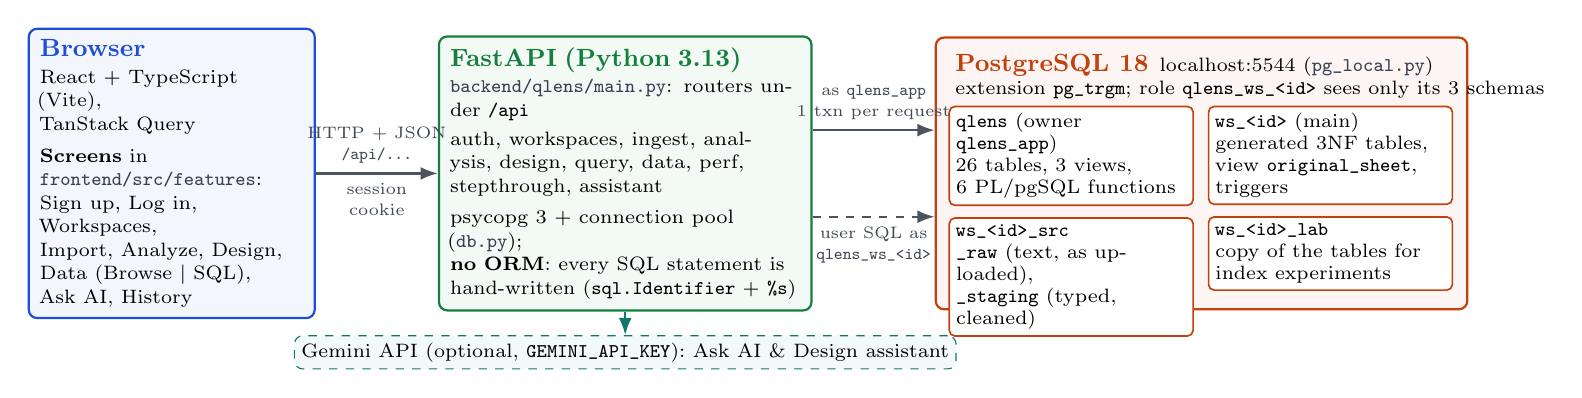
\begin{tikzpicture}[
    font=\fontsize{7.2}{8.5}\selectfont,
    sch/.style={draw=#1, fill=white, line width=0.6pt, rounded corners=2pt, align=left, inner sep=2.5pt,
      text width=2.92cm, font=\fontsize{6.7}{7.9}\selectfont},
    arr/.style={-{Latex[length=2.2mm]}, line width=0.8pt, draw=ink!80},
    lab/.style={font=\fontsize{6.4}{7.5}\selectfont, align=center, text=ink!85},
  ]
  % client
  \node[draw=cIntro, fill=cIntro!5, line width=0.8pt, rounded corners=3pt, align=left, inner sep=4pt,
        text width=3.35cm, minimum height=3.45cm] (web) at (0,0) {%
    {\bfseries\fontsize{8.6}{10}\selectfont\color{cIntro} Browser}\\[1pt]
    React + TypeScript (Vite),\\ TanStack Query\\[3pt]
    \textbf{Screens} in\\ \fn{frontend/src/features}:\\
    Sign up, Log in, Workspaces,\\ Import, Analyze, Design,\\ Data (Browse \textbar{} SQL),\\ Ask AI, History};
  % server
  \node[draw=cSql, fill=cSql!5, line width=0.8pt, rounded corners=3pt, align=left, inner sep=4pt,
        text width=4.45cm, minimum height=3.45cm, right=1.55cm of web] (api) {%
    {\bfseries\fontsize{8.6}{10}\selectfont\color{cSql} FastAPI (Python 3.13)}\\[1pt]
    \fn{backend/qlens/main.py}: routers under \cd{/api}\\[2pt]
    auth, workspaces, ingest, analysis, design, query, data, perf, stepthrough, assistant\\[3pt]
    psycopg 3 + connection pool (\fn{db.py});\\ \textbf{no ORM}: every SQL statement is\\ hand-written
    (\cd{sql.Identifier} + \texttt{\%s})};
  % database
  \node[draw=cAdv, fill=cAdv!5, line width=0.8pt, rounded corners=3pt, inner sep=0pt,
        minimum width=6.75cm, minimum height=3.45cm, right=1.55cm of api] (pg) {};
  \node[anchor=north west, align=left, font=\fontsize{6.9}{8.2}\selectfont] at ($(pg.north west)+(4pt,-3pt)$)
    {{\bfseries\fontsize{8.6}{10}\selectfont\color{cAdv} PostgreSQL 18}\enspace localhost:5544 (\fn{pg_local.py})\\
     extension \cd{pg_trgm}; role \cd{qlens_ws_<id>} sees only its 3 schemas};
  \node[sch=cAdv, anchor=north west] (s1) at ($(pg.north west)+(5pt,-25pt)$)
    {{\bfseries\cd{qlens}} (owner \cd{qlens_app})\\ 26 tables, 3 views,\\ 6 PL/pgSQL functions};
  \node[sch=cAdv, anchor=north west] (s2) at ($(s1.north east)+(5pt,0)$)
    {{\bfseries\cd{ws_<id>}} (main)\\ generated 3NF tables,\\ view \cd{original_sheet}, triggers};
  \node[sch=cAdv, anchor=north west] (s3) at ($(s1.south west)+(0,-4pt)$)
    {{\bfseries\cd{ws_<id>_src}}\\ \cd{_raw} (text, as uploaded),\\ \cd{_staging} (typed, cleaned)};
  \node[sch=cAdv, anchor=north west] (s4) at ($(s2.south west)+(0,-4pt)$)
    {{\bfseries\cd{ws_<id>_lab}}\\ copy of the tables for\\ index experiments};
  % arrows
  \draw[arr] (web.east) -- node[lab, above] {HTTP + JSON\\ \cd{/api/...}} node[lab, below] {session\\ cookie} (api.west);
  \draw[arr] ($(api.east)+(0,0.55)$) -- node[lab, above] {as \cd{qlens_app}\\ 1 txn per request} ($(pg.west)+(0,0.55)$);
  \draw[arr, dashed] ($(api.east)+(0,-0.55)$) -- node[lab, below] {user SQL as\\ \cd{qlens_ws_<id>}} ($(pg.west)+(0,-0.55)$);
  % optional Gemini
  \node[draw=cOpt, dashed, fill=cOpt!5, rounded corners=3pt, font=\fontsize{6.7}{8}\selectfont, align=center,
        inner sep=2.5pt, below=0.3cm of api] (gem) {Gemini API (optional, \cd{GEMINI_API_KEY}): Ask AI \& Design assistant};
  \draw[arr, dashed, draw=cOpt] (api.south) -- (gem.north);
\end{tikzpicture}
\end{center}
\vspace{-6pt}



\begin{multicols}{2}

\begin{topic}[cOpt]{Which DBMS and libraries}
\begin{itemize}
  \item \textbf{PostgreSQL 18}, run as a private local cluster (\fn{backend/.pgdata}, port 5544) by
  \fn{pg_local.py} (\code{initdb}, \code{pg_ctl}); databases \code{qlens} and \code{qlens_test} (pytest).
  \item \textbf{psycopg 3} driver + \code{psycopg_pool}; \textbf{no ORM}. \textbf{pglast} = PostgreSQL's
  own parser, used to check typed SQL and split it for step-through. \textbf{pg\_trgm} =
  \code{similarity()}, the \code{%} operator and GIN trigram indexes.
  \item Migrations \fn{backend/sql/migrations/000}--\fn{008} run in order by \fn{migrate.py}:
  000 bootstrap \textperiodcentered{} 001 tables, constraints, indexes \textperiodcentered{} 002 triggers + views
  \textperiodcentered{} 003 \code{try_date} \textperiodcentered{} 004 \code{check_fd}, \code{is_unique}
  \textperiodcentered{} 005 assistant tables, design versions \textperiodcentered{} 006 \code{row_changes} +
  audit trigger \textperiodcentered{} 007 SECURITY DEFINER, REVOKE \textperiodcentered{} 008 \code{has_renames}.
\end{itemize}
\end{topic}

\begin{topic}[cOpt]{Per-workspace schemas (the user's data)}
\begin{itemize}
  \item {\bfseries\code{ws_<id>_src}}: \code{_raw} = every sheet column as \code{text}
  (+ \code{_row_id} PK), loaded by \code{COPY}, never changed; \code{_staging} = typed copy
  (\code{CREATE TABLE AS SELECT}) that clean-up edits and analysis reads.
  \item {\bfseries\code{ws_<id>}} (main): the applied tables, for the fee register:
\end{itemize}
{\fontsize{7.1}{8.6}\selectfont\ttfamily
\hspace*{0.8em}teachers(\underline{id}, teacher U, teacher\_phone U)\\
\hspace*{0.8em}batches(\underline{id}, batch U, \textit{teacher\_id}$\to$teachers)\\
\hspace*{0.8em}students(\underline{id}, student\_name U, student\_phone U,\\
\hspace*{0.8em}\phantom{students(}\textit{batch\_id}$\to$batches)\\
\hspace*{0.8em}fee\_register(\underline{id}, \textit{student\_id}$\to$students, month, fee\_paid,\\
\hspace*{0.8em}\phantom{fee\_register(}payment\_mode; U(student\_id, month))\par}
\hspace*{0.95em}plus view \code{original_sheet} and trigger \code{log_row_change} on each table
(U = UNIQUE; FKs are \code{ON DELETE RESTRICT}).
\begin{itemize}
  \item {\bfseries\code{ws_<id>_lab}}: copy of the applied tables
  (\code{CREATE TABLE ... (LIKE ...)}) for Explain \& speed up and ``scale $\times$N'';
  rebuilt after each Apply (\fn{perf/lab.py:ensure_lab L123}).
\end{itemize}
\end{topic}

\end{multicols}

\begin{topic}[cOpt]{ER sketch of the \code{qlens} schema (textbook notation, main entities)}
\centering
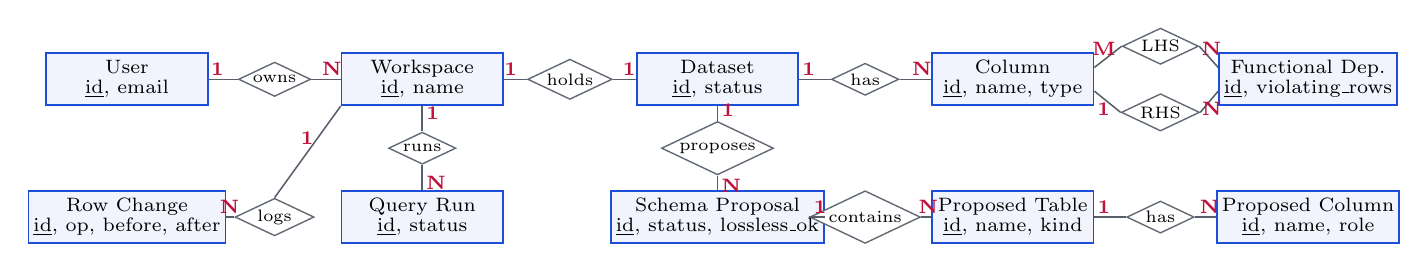
\begin{tikzpicture}[
    font=\fontsize{7}{8}\selectfont,
    ent/.style={draw=cIntro, fill=cIntro!6, line width=0.6pt, minimum width=2.05cm, minimum height=0.66cm,
      align=center, inner sep=1.8pt},
    rel/.style={diamond, aspect=2.1, draw=ink!70, fill=white, line width=0.5pt, inner sep=0.8pt,
      font=\fontsize{6.4}{7.2}\selectfont},
    ln/.style={line width=0.55pt, draw=ink!75},
    c/.style={font=\bfseries\fontsize{6.8}{7.6}\selectfont, text=cNorm, inner sep=1.2pt},
  ]
  \def\dx{3.75}
  \def\dy{1.75}
  % entity sets (key attribute underlined)
  \node[ent] (U) at (0,0) {User\\[-1pt]\underline{id}, email};
  \node[ent] (W) at (\dx,0) {Workspace\\[-1pt]\underline{id}, name};
  \node[ent] (D) at (2*\dx,0) {Dataset\\[-1pt]\underline{id}, status};
  \node[ent] (C) at (3*\dx,0) {Column\\[-1pt]\underline{id}, name, type};
  \node[ent] (F) at (4*\dx,0) {Functional Dep.\\[-1pt]\underline{id}, violating\_rows};
  \node[ent] (R) at (0,-\dy) {Row Change\\[-1pt]\underline{id}, op, before, after};
  \node[ent] (Q) at (\dx,-\dy) {Query Run\\[-1pt]\underline{id}, status};
  \node[ent] (P) at (2*\dx,-\dy) {Schema Proposal\\[-1pt]\underline{id}, status, lossless\_ok};
  \node[ent] (T) at (3*\dx,-\dy) {Proposed Table\\[-1pt]\underline{id}, name, kind};
  \node[ent] (K) at (4*\dx,-\dy) {Proposed Column\\[-1pt]\underline{id}, name, role};
  % relationship sets with cardinalities
  \node[rel] (owns) at (0.5*\dx,0) {owns};
  \draw[ln] (U) -- node[c, above, pos=0.3] {1} (owns); \draw[ln] (owns) -- node[c, above, pos=0.7] {N} (W);
  \node[rel] (holds) at (1.5*\dx,0) {holds};
  \draw[ln] (W) -- node[c, above, pos=0.3] {1} (holds); \draw[ln] (holds) -- node[c, above, pos=0.7] {1} (D);
  \node[rel] (has) at (2.5*\dx,0) {has};
  \draw[ln] (D) -- node[c, above, pos=0.3] {1} (has); \draw[ln] (has) -- node[c, above, pos=0.7] {N} (C);
  \node[rel] (lhs) at (3.5*\dx,0.42) {LHS};
  \draw[ln] ($(C.east)+(0,0.15)$) -- node[c, above, pos=0.35] {M} (lhs.west);
  \draw[ln] (lhs.east) -- node[c, above, pos=0.65] {N} ($(F.west)+(0,0.15)$);
  \node[rel] (rhs) at (3.5*\dx,-0.42) {RHS};
  \draw[ln] ($(C.east)+(0,-0.15)$) -- node[c, below, pos=0.35] {1} (rhs.west);
  \draw[ln] (rhs.east) -- node[c, below, pos=0.65] {N} ($(F.west)+(0,-0.15)$);
  \node[rel] (logs) at (0.5*\dx,-\dy) {logs};
  \draw[ln] (W.south west) -- node[c, left, pos=0.35] {1} (logs.north); \draw[ln] (logs) -- node[c, above, pos=0.6] {N} (R);
  \node[rel] (runs) at (\dx,-0.5*\dy) {runs};
  \draw[ln] (W) -- node[c, right, pos=0.3] {1} (runs); \draw[ln] (runs) -- node[c, right, pos=0.7] {N} (Q);
  \node[rel] (prop) at (2*\dx,-0.5*\dy) {proposes};
  \draw[ln] (D) -- node[c, right, pos=0.3] {1} (prop); \draw[ln] (prop) -- node[c, right, pos=0.7] {N} (P);
  \node[rel] (cont) at (2.5*\dx,-\dy) {contains};
  \draw[ln] (P) -- node[c, above, pos=0.3] {1} (cont); \draw[ln] (cont) -- node[c, above, pos=0.7] {N} (T);
  \node[rel] (hasc) at (3.5*\dx,-\dy) {has};
  \draw[ln] (T) -- node[c, above, pos=0.3] {1} (hasc); \draw[ln] (hasc) -- node[c, above, pos=0.7] {N} (K);
\end{tikzpicture}\par
\raggedright
Rectangles = entity sets, diamonds = relationship sets, 1/N/M = cardinality. LHS is M\,:\,N because a
dependency may have two columns on its left side (table \code{fd_lhs_columns}). Not drawn: Saved Query
1\,:\,N Query Run, Candidate Key M\,:\,N Column, Proposed Column \emph{refers to} Proposed Table, the 3
assistant tables.
\end{topic}


% ---- metadata tables ----------------------------------------------------------------------------
\begin{topic}[cOpt]{The 26 tables of schema \code{qlens}: keys and references\hfill
  {\mdseries\fontsize{6.9}{8}\selectfont PK underlined \textperiodcentered{} U = UNIQUE \textperiodcentered{}
  C = ON DELETE CASCADE \textperiodcentered{} N = SET NULL \textperiodcentered{} \cd{x_id} refers to table \cd{xs} unless named}}
{\fontsize{6.8}{8.0}\selectfont\renewcommand{\arraystretch}{1.0}\setlength{\tabcolsep}{2.2pt}%
\begin{minipage}[t]{0.488\linewidth}
\begin{tabularx}{\linewidth}[t]{@{}>{\ttfamily}l >{\raggedright\arraybackslash}X >{\raggedright\arraybackslash}p{2.75cm}@{}}
\toprule
\normalfont\bfseries table & \bfseries keys & \bfseries references\\
\midrule
\multicolumn{3}{@{}l}{\color{cOpt}\bfseries Accounts}\\
users & \underline{id}; U(email) & --\\
sessions & \underline{token\_hash} & user\_id C\\
workspaces & \underline{id}; U(owner\_id, name) & owner\_id$\to$users C\\
\multicolumn{3}{@{}l}{\color{cOpt}\bfseries Imported sheet}\\
datasets & \underline{id}; U(workspace\_id): 1\,:\,1 & workspace\_id C\\
dataset\_columns & \underline{id}; U(dataset\_id, name), U(dataset\_id, ordinal) & dataset\_id C\\
\multicolumn{3}{@{}l}{\color{cOpt}\bfseries Analysis}\\
candidate\_keys & \underline{id} & dataset\_id C\\
candidate\_key\_columns & \underline{key\_id, column\_id}: M\,:\,N & key\_id C, column\_id C\\
functional\_dependencies & \underline{id} & dataset\_id C, rhs\_column\_id C\\
fd\_lhs\_columns & \underline{fd\_id, column\_id}: M\,:\,N & fd\_id C, column\_id C\\
duplicate\_groups & \underline{id}; U(dataset\_id, column\_id, canonical\_value) & dataset\_id C, column\_id C\\
duplicate\_values & \underline{group\_id, value}: weak entity & group\_id C\\
dataset\_fixes & \underline{id} & dataset\_id C, column\_id C\\
row\_changes & \underline{id} (written by the trigger) & workspace\_id C\\
\bottomrule
\end{tabularx}
\end{minipage}\hfill
\begin{minipage}[t]{0.488\linewidth}
\begin{tabularx}{\linewidth}[t]{@{}>{\ttfamily}l >{\raggedright\arraybackslash}X >{\raggedright\arraybackslash}p{2.75cm}@{}}
\toprule
\normalfont\bfseries table & \bfseries keys & \bfseries references\\
\midrule
\multicolumn{3}{@{}l}{\color{cOpt}\bfseries Designs}\\
schema\_proposals & \underline{id}; partial U: 1 draft + 1 applied & dataset\_id C, based\_on\_id N\\
proposed\_tables & \underline{id}; U(proposal\_id, name) & proposal\_id C\\
proposed\_columns & \underline{id}; U(table\_id, name) & table\_id C, references\_table\_id C, source\_column\_id N\\
proposed\_unique\_keys & \underline{id} & table\_id C\\
proposed\_unique\_key\_columns & \underline{key\_id, column\_id}: M\,:\,N & key\_id C, column\_id C\\
\multicolumn{3}{@{}l}{\color{cOpt}\bfseries Queries and performance}\\
saved\_queries & \underline{id}; U(workspace\_id, title) & workspace\_id C\\
query\_runs & \underline{id} & workspace\_id C, saved\_query\_id N\\
nl\_questions & \underline{id}; U(query\_run\_id) & query\_run\_id C (not yet written)\\
explain\_snapshots & \underline{id} & workspace\_id C, query\_run\_id C\\
index\_experiments & \underline{id} & workspace\_id C\\
\multicolumn{3}{@{}l}{\color{cOpt}\bfseries Assistant (optional)}\\
assistant\_conversations & \underline{id} & workspace\_id C\\
assistant\_messages & \underline{id}; U(conversation\_id, seq) & conversation\_id C\\
assistant\_tool\_calls & \underline{id}; U(message\_id, seq) & message\_id C, query\_run\_id N\\
\bottomrule
\end{tabularx}
\end{minipage}\par}
\smallskip
{\fontsize{6.9}{8.2}\selectfont Named parents: \code{rhs_column_id}, \code{source_column_id}, \code{column_id}
$\to$ \code{dataset_columns} (in \code{proposed_unique_key_columns}: $\to$ \code{proposed_columns}); \code{owner_id} $\to$ \code{users}; \code{based_on_id} $\to$ \code{schema_proposals};
\code{table_id}, \code{references_table_id} $\to$ \code{proposed_tables}; \code{key_id} $\to$ \code{candidate_keys} /
\code{proposed_unique_keys}; \code{fd_id} $\to$ \code{functional_dependencies}; \code{group_id} $\to$
\code{duplicate_groups}; \code{message_id} $\to$ \code{assistant_messages}.}
\end{topic}

% ---- request walkthroughs -----------------------------------------------------------------------
\begin{multicols}{2}

\begin{topic}[ink]{Walkthrough 0: create a workspace (dashboard)}
\begin{enumerate}
  \item \code{POST /api/workspaces} $\to$ \fn{workspaces/service.py:create_workspace L71}.
  \item \code{INSERT INTO qlens.workspaces ... ON CONFLICT (owner_id, name) DO NOTHING RETURNING id}.
  \item \code{CREATE ROLE qlens_ws_<id> ...}, \code{ALTER ROLE ... SET ...}, \code{CREATE SCHEMA} + GRANTs
  for \code{ws_<id>} and \code{ws_<id>_src}, all in the same transaction.
  \item List: \code{GET /api/workspaces} reads \code{qlens.v_workspace_summary}. Delete drops the 3
  schemas, \code{DROP OWNED BY}, \code{DROP ROLE}, then the row (cascades).
\end{enumerate}
\end{topic}

\begin{topic}[ink]{Walkthrough 1: Import}
\begin{enumerate}
  \item \ic|POST /api/workspaces/{id}/dataset| (file) or \code{/dataset/sample} $\to$
  \fn{ingest/routes.py:upload_dataset}, \fn{import_sample}.
  \item \fn{ingest/parse.py:read_table}: CSV/XLSX $\to$ rows; headers become safe names (\fn{sanitize_names}).
  \item \fn{ingest/stage.py:import_dataset L62}, one transaction: \fn{_reset_workspace} (DELETE old
  dataset, cascades; DROP/CREATE schemas) $\to$ \fn{_load_raw} (CREATE TABLE \code{_raw}, COPY) $\to$
  \fn{_infer_type} $\to$ \fn{_build_staging} $\to$ \fn{_record} (INSERT \code{datasets},
  \code{dataset_columns} with null/distinct counts).
  \item \code{GET .../dataset} shows the first 50 rows of \code{_staging}.
\end{enumerate}
\end{topic}

\begin{topic}[ink]{Walkthrough 2: Analyze (and clean-up)}
\begin{enumerate}
  \item \code{POST .../analyze} $\to$ \fn{analysis/discover.py:analyze L155}, one transaction.
  \item DELETE old keys/FDs; \fn{_find_keys} (\code{qlens.is_unique}), \fn{_find_fds}
  (\code{qlens.check_fd}) $\to$ INSERT \code{candidate_keys}, \code{candidate_key_columns},
  \code{functional_dependencies}, \code{fd_lhs_columns}.
  \item \fn{cleanup.py:find_duplicates}: \code{similarity()} + GIN trigram index $\to$
  \code{duplicate_groups}, \code{duplicate_values}.
  \item \code{UPDATE qlens.datasets SET status = 'analyzed'}.
  \item Fixes: \ic|POST .../duplicates/{g}/merge|, \ic|.../inconsistencies/{fd}/fix|,
  \code{.../cleanup/accept-all} $\to$ UPDATE \code{_staging} (FOR UPDATE), INSERT \code{dataset_fixes},
  re-analyze in the same transaction. \ic|PATCH .../fds/{id}| sets \code{accepted}.
\end{enumerate}
\end{topic}

\begin{topic}[ink]{Walkthrough 3: Design}
\begin{enumerate}
  \item \code{POST .../proposal} $\to$ \fn{design/proposal.py:build L186}.
  \item \fn{discover.load_fds} $\to$ \fn{to_algebra} (exact, accepted, not derived) $\to$
  \fn{fd_algebra.synthesize_3nf} $\to$ \fn{_plan} (names, \code{id}, FKs, UNIQUE keys).
  \item Transaction: old draft $\to$ \code{'superseded'}; INSERT \code{schema_proposals},
  \code{proposed_tables}, \code{proposed_columns}, \code{proposed_unique_keys} (+ \code{_columns}).
  \item Renames: \ic|PATCH .../proposal/tables/{id}|, \ic|.../columns/{id}| (row lock
  \code{FOR UPDATE}). SQL panel: \code{GET .../proposal/sql} $\to$ \fn{ddl.render} + \fn{ddl.as_text}.
\end{enumerate}
\end{topic}

\begin{topic}[ink]{Walkthrough 4: Apply design}
\begin{enumerate}
  \item \code{POST .../apply} $\to$ \fn{design/apply.py:apply_proposal L67}.
  \item One transaction: lock the draft (\code{FOR UPDATE}); \code{DROP SCHEMA ws_<id>_lab, ws_<id> CASCADE};
  \code{CREATE SCHEMA}; run \fn{ddl.render}: CREATE TABLE (parents first), INSERT \dots{} SELECT,
  CREATE TRIGGER, CREATE VIEW \code{original_sheet}, verify (EXCEPT ALL).
  \item Rows differ $\to$ 409 \code{lossless_check_failed} with sample rows, ROLLBACK: old tables stay.
  \item Else UPDATE \code{schema_proposals} (old applied $\to$ superseded, this $\to$ applied,
  \code{lossless_ok = true}), \code{datasets.status = 'applied'}; then \code{ANALYZE} each table.
\end{enumerate}
\end{topic}

\begin{topic}[ink]{Walkthrough 5: Data $>$ Browse}
\begin{enumerate}
  \item \ic|GET .../data/{table}?page&sort&dir&q&f| $\to$ \fn{data/service.py:list_rows L243}:
  \code{SELECT count(*)} + \code{SELECT ... WHERE ... ORDER BY ... LIMIT %s OFFSET %s}.
  \item \code{POST}/\code{PATCH}/\ic|DELETE .../data/{table}[/{row_id}]| $\to$ \fn{insert_row},
  \fn{update_row}, \fn{delete_row} inside a savepoint (\fn{_guarded}); a constraint error $\to$
  \fn{_explain} reads \code{pg_constraint} and returns a ``constraint card''.
  \item Trigger $\to$ \code{qlens.row_changes}; \code{GET .../data-changes} = audit timeline. Also
  \code{/related} (rows pointing here), \code{/export} (CSV), \code{/options} (FK picker).
\end{enumerate}
\end{topic}

\begin{topic}[ink]{Walkthrough 6: Data $>$ SQL}
\begin{enumerate}
  \item SELECT: \code{POST .../query} $\to$ \fn{query/routes.py:run_query L162} $\to$
  \fn{validate_select} $\to$ \fn{sandbox.run} (role, READ ONLY, cursor) $\to$ \fn{record_run}:
  INSERT \code{qlens.query_runs} (trigger updates \code{saved_queries}).
  \item Write (after the confirm dialog): \code{POST .../query/write} $\to$ \fn{validate_write} $\to$
  \fn{sqlwrite.writable_table} $\to$ \fn{sandbox.run_write} (READ WRITE, COMMIT); audit trigger fires.
  \item \code{POST .../stepthrough} $\to$ \fn{stages.run_stages}. \code{POST .../explain} $\to$
  \code{EXPLAIN (ANALYZE, BUFFERS, FORMAT JSON)}, \code{explain_snapshots}, \fn{advisor.suggest};
  \code{POST .../lab/try-index} $\to$ \fn{lab.try_index}.
\end{enumerate}
\end{topic}

\begin{topic}[ink]{Walkthrough 7: Ask AI \hfill\opt}
\begin{enumerate}
  \item \code{POST .../assistant} (\code{context 'data'}) $\to$ \fn{assistant/service.py:respond L134}.
  \item INSERT \code{assistant_conversations} (new chat) and the user's \code{assistant_messages} row.
  \item Up to 6 rounds: Gemini (\fn{assistant/llm.py}) asks for tools $\to$ \fn{tools.execute}, e.g.\
  \code{run_sql} = \fn{validate_select} + \fn{sandbox.run} + a \code{query_runs} row (\code{source 'english'}).
  \item INSERT the reply + \code{assistant_tool_calls}. A Gemini error rolls the whole turn back
  (429 = rate limit).
\end{enumerate}
\end{topic}

\begin{topic}[ink]{Walkthrough 8: History}
\begin{enumerate}
  \item \code{GET .../history} $\to$ \code{SELECT ... FROM qlens.query_runs WHERE workspace_id = %s
  ORDER BY created_at DESC, id DESC LIMIT %s} (uses \code{query_runs_workspace_time_idx}).
  \item \code{GET .../slow-queries} $\to$ \code{v_slow_queries}; \code{.../saved-queries} (CRUD) $\to$
  \code{saved_queries}; \ic|.../saved-queries/{id}/trend| $\to$ \code{v_saved_query_trend}.
\end{enumerate}
\end{topic}

% ---- file map -----------------------------------------------------------------------------------
\begin{topic}[cOpt]{File map: \cd{backend/qlens/}}
\setlength{\parskip}{0.6pt}
\fn{main.py} FastAPI app, routers under \code{/api}, opens/closes the pool.\\
\fn{config.py} settings from \fn{.env} (database URL, secret key, optional Gemini key).\\
\fn{db.py} pool; \fn{get_conn} = 1 transaction per request; workspace role/schema helpers, GRANTs.\\
\fn{pg_local.py} private PostgreSQL 18 cluster (init/start/stop/status). \fn{setup_db.py} role
\code{qlens_app}, databases, \code{pg_trgm}. \fn{migrate.py} runs the migrations. \fn{errors.py}
\code{ApiError} $\to$ JSON error.\\
\fn{auth/} sign-up, log-in, sessions; \fn{deps.py}: \fn{current_user}, \fn{owned_workspace}.\\
\fn{workspaces/} create (role + schemas), list (view), delete.\\
\fn{ingest/} \fn{parse.py} CSV/XLSX; \fn{stage.py} \code{_raw}, \code{_staging}, types, profile.\\
\fn{samples/generate.py} 3 sample sheets with planted mistakes.\\
\fn{analysis/} \fn{discover.py} keys + FDs; \fn{fd_algebra.py} closure, canonical cover, 3NF;
\fn{cleanup.py} duplicates, fixes.\\
\fn{design/} \fn{proposal.py} build/store/rename/versions; \fn{naming.py} table names; \fn{ddl.py}
the SQL script; \fn{apply.py} run it + lossless check; \fn{catalog.py} reads \code{pg_catalog}.\\
\fn{query/} \fn{validate.py} SQL checks (pglast); \fn{sandbox.py} role connection, cursor, timeouts;
\fn{routes.py} run, write, history, saved queries; \fn{serialize.py} values $\to$ JSON.\\
\fn{data/} \fn{service.py} Browse rows, edits, related rows, CSV, audit log; \fn{sqlwrite.py} typed writes.\\
\fn{perf/} \fn{explain.py} plan tree; \fn{advisor.py} index suggestions; \fn{lab.py} lab copy, scale, try index.\\
\fn{stepthrough/stages.py} SELECT $\to$ algebra stages. \fn{assistant/} \fn{llm.py} Gemini client,
\fn{tools.py} the 10 tools, \fn{service.py} chat loop + undo.\\
\fn{backend/tests/} 26 pytest files against a real PostgreSQL test database (e.g.\
\fn{test_fd_algebra.py}, \fn{test_apply.py}, \fn{test_sandbox.py}, \fn{test_validate.py}).\\[2pt]
{\color{cOpt}\bfseries Frontend} \fn{frontend/src/features/}: \fn{auth}, \fn{workspaces} (dashboard,
step rail), \fn{import}, \fn{analyze}, \fn{design} (ER canvas, SQL panel, Apply), \fn{data} (Browse, SQL
tab, constraint cards), \fn{query} (editor, results, step-through), \fn{perf} (plan, before/after),
\fn{assistant} (Ask AI, design assistant), \fn{history}; \fn{lib/api.ts} = fetch wrapper.
\end{topic}

% ---- viva answers -------------------------------------------------------------------------------
\begin{topic}[cNorm]{Viva quick answers}
\setlength{\parskip}{2pt}
\textbf{Why surrogate keys (\code{id})?} A short number that never changes when a name is corrected, so
foreign keys never need updating and joins use one column. The natural key is still enforced by UNIQUE.

\textbf{How do you prove the decomposition is lossless?} Theory: each join is on a key of one side and
one table holds a candidate key. Practice: Apply rebuilds the sheet with \code{original_sheet} and runs
EXCEPT ALL both ways; both counts must be 0, else ROLLBACK.

\textbf{How do you stop SQL injection?} Values are bound parameters (\code{%s}); names go through
\code{sql.Identifier} / \code{format('%I')}; typed SQL must parse as one SELECT and runs as a role that can
read only its own workspace.

\textbf{Why a trigger for the audit log?} The database records every change from every path (forms,
typed SQL) in the same transaction; code cannot forget it, and a rolled-back change leaves no log row.

\textbf{What is the cursor for?} The sandbox DECLAREs a cursor for the user's SELECT and FETCHes at most
1{,}001 rows, so a huge result never fills memory; the 1{,}001st row only signals ``truncated''.

\textbf{Why compute a canonical cover first?} It removes redundant FDs and extra left-side columns, so the
3NF algorithm makes no needless tables (no table for student\_name $\to$ teacher).

\textbf{Why 3NF and not BCNF?} 3NF synthesis is always lossless \emph{and} dependency preserving; BCNF
can lose dependency preservation. The fee register tables are in BCNF anyway.

\textbf{Where are FDs found: Python or SQL?} In SQL: \code{qlens.check_fd} groups the rows inside
PostgreSQL. Python only chooses which columns to test and runs closure, cover and synthesis on the small
list of FDs.

\textbf{Two people click Apply at once?} The draft row is locked with \code{SELECT ... FOR UPDATE}; the
second waits, sees \code{'applied'} and gets 409. Partial unique indexes allow one draft and one applied
design per dataset.

{\bfseries Why \code{lossless_ok IS TRUE} in the CHECK?} A CHECK passes on NULL; \code{IS TRUE} makes
``not checked yet'' (NULL) fail.

\textbf{Why one schema and role per workspace?} Isolation and least privilege: a user's SQL can see
only their own tables, and \code{DROP SCHEMA ... CASCADE} removes a workspace in one statement.

\textbf{What happens on a constraint error in Browse?} Only the savepoint is rolled back; QLens reads
\code{pg_constraint} and shows which rule (UNIQUE, FOREIGN KEY, NOT NULL, CHECK) refused the change.
\end{topic}

\begin{topic}[cSql]{Demo order for the viva (from the README)}
\begin{enumerate}
  \item Sign up $\to$ dashboard $\to$ \textbf{Try a sample} $\to$ fee register (3{,}000 rows).
  \item \textbf{Analyze}: exact FDs (student\_name $\to$ batch, batch $\to$ teacher), the candidate key,
  inconsistencies (student\_phone $\to$ student\_name broken by 8 rows) $\to$ fix $\to$ \textbf{Accept all}.
  \item \textbf{Design}: the 3NF tables on the ER canvas; rename a table; \textbf{Apply design} $\to$
  lossless check (EXCEPT ALL both ways = 0 rows).
  \item \textbf{Data $>$ Browse}: add a student with an existing name (UNIQUE card); delete a student who
  has fee rows (FOREIGN KEY card, \code{ON DELETE RESTRICT}). In \textbf{Data $>$ SQL}, confirm:
\end{enumerate}
\begin{sqlc}
INSERT INTO fee_register (student_id, month, fee_paid, payment_mode)
VALUES (999999, 'Apr', 4000, 'UPI');      -- no student 999999: FK card
\end{sqlc}
\begin{enumerate}[resume]
  \item \textbf{Data $>$ SQL}: a join; \code{SELECT * FROM fee_register WHERE fee_paid = 2100} $\to$
  \textbf{Explain \& speed up} (Seq Scan, try the index); a GROUP BY query $\to$ \textbf{Step through};
  an UPDATE with the confirm dialog.
  \item \textbf{Ask AI} (needs the Gemini key, else it says why it is off), then \textbf{History}.
\end{enumerate}
\end{topic}


\end{multicols}

\end{document}
